\chapter{IPv6-SLAAC}
\label{chap:ipv6_slaac}

\section{Ejercicio 2.1}
\subsection{Muestra una captura del escenario en el momento inicial de la simulación en la que se vean todas las
direcciones MAC e IP. Utilizando la dirección IP de host[0] como ejemplo, explica cómo se construye, destacando
los campos y bits relevantes. Utiliza para explicarlo la notación IPv6 no abreviada (16 bytes:
xxxx:xxxx:xxxx:xxxx:xxxx:xxxx:xxxx:xxxx)}

\begin{figure}[!ht]
    \centering
    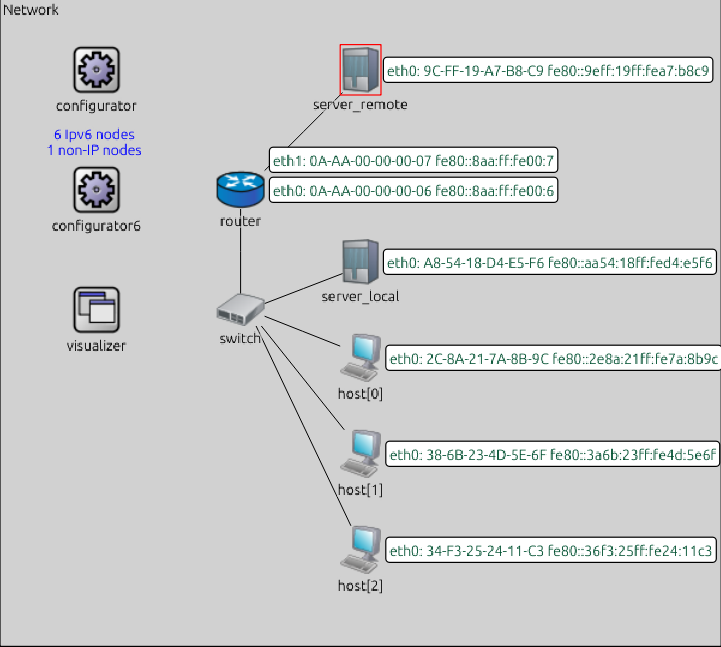
\includegraphics[width=135mm, scale=0.75]{imaxes/captura_ejer2_1.png}
    \caption{Escenario inicial dispositivos con IPv6}
    \label{fig:direccion_ipv6_host0}
\end{figure}

En el principio de la simulación, las direcciones que se muestran son direcciones unicast local de enlace. Estas son direcciones se generan automáticamente una vez que un dispositivo se conecta a una red. La estructura de este tipo de direcciones tienen como prefijo FE80::, no se enrutan y son únicas en ese enlace específico.

La segunda parte de la dirección se forma a partir de la dirección MAC del dispositivo. Para esto, fijamos el séptimo bit a 1 e insertamos 0XFFFE entre las dos mitades de la dirección MAC del dispositivo. 

Como ejemplo, vamos a ver la dirección unicast local de enlace que genera el dispositivo host[0]. Como vemos en la imagen \ref{fig:direccion_ipv6_host0}, su dirección está formada por el prefijo FE80:: y, después, 2E8A:21FF:FE7A:8B9C. Esa segunda parte, como se explicó antes, se forma a partir de su dirección MAC (2C-8A-21-7A-8B-9C). Como se puede observar, en los primeros 2 bytes de la dirección unicast local de enlace (2E8A), si lo comparamos con su dirección MAC, el segundo carácter se convierte en una E, ya que tenemos que añadir un uno en el séptimo bit (La letra C hexadecimal, que en binario es 1100, como su tercer bit corresponde al séptimo bit de la dirección unicast, pasa a ser 1 por lo que se convierte en E -> 1110). Llegados a este punto, tras el primer cambio, tenemos la siguiente estructura -> FE80::2E80:21.

Como se explicó anteriormente, una vez hecho el primer cambio, ahora añadimos 0XFFFE  y posteriormente los últimos 3 bytes de la dirección MAC, por lo que queda como dirección final unicast local de enlace\\ FE80::2E8A:21FF:FE7A:8B9C.


\section{Ejercicio 2.2}\label{chap:ejer22}
\subsection{Asigna al host[2] la misma dirección MAC que al host[0] y arranca la simulación. ¿Qué error ocurre antes de
que haya transcurrido el primer segundo de simulación? Muestra una captura del error que aparece. ¿Qué
paquete (tipo, origen y destino) provoca el error? ¿Por qué?}

\begin{figure}[!ht]
    \centering
    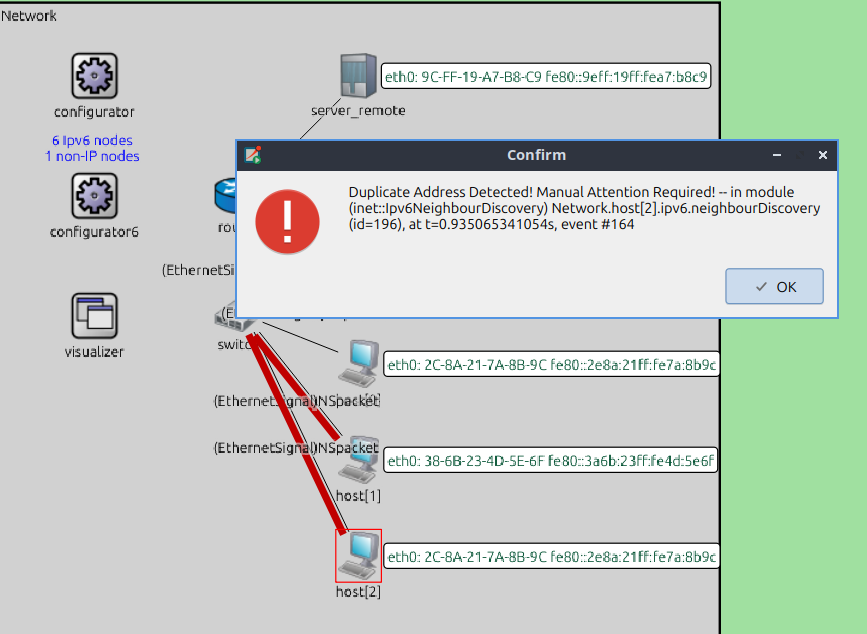
\includegraphics[width=135mm, scale=0.75]{imaxes/captura_ejer2_2.png}
    \caption{Fallo en la red con MAC host[2] igual a la de host[0]}
    \label{fig:fallo_ipv6_host2}
\end{figure}

Tal y como se muestra en la imagen \ref{fig:fallo_ipv6_host2}, hay un fallo de direcciones duplicadas cuando el host[2] intenta asignarse una dirección IPv6. 

El paquete en concreto que provoca el error es de tipo ICMPv6 con mensaje NS (Neighbor Solicitation), donde el origen de momento es el host[2] (En ese momento sin ninguna dirección) y como destino una dirección multicast. Este error ocurre porque el host[2], cuando crea su dirección, le comunica a sus vecinos de la red (DAD) cómo es su dirección.Entonces, se encuentra que el host[0] tiene la misma dirección IPv6 que él se asignó, por lo que ocurre un conflicto de IPs.

\section{Ejercicio 2.3}
\subsection{Cambia la MAC del host[2] de manera que coincida con la de host[0] en los últimos 3 bytes y difiera en los 3
primeros bytes (mantén esta MAC para el resto de las cuestiones). Asigna a serverremote la misma MAC que a
host[0]. ¿Vuelve a ocurrir el error de dirección duplicada con serverremote y host[0]? ¿Por qué?}

En este caso, al poner la misma MAC al host[0] y al server remote no produce ningún error porque son dispositivos que están en diferentes redes. 
El conflicto que sucedía en el ejercicio \ref{chap:ejer22} sucede porque los dos dispositivos estaban en la misma red, por lo que salta el error de 
direcciones duplicadas. Esto ocurre igual que en IPv4 con las IPs privadas: En la misma red no puede haber dos IPs iguales, pero si hay dos redes diferentes, puede coincidir una IP privada de un dispositivo que está en la red1 con la IP de otro dispositivo que esté en la red2.

\section{Ejercicio 2.4}
\subsection{¿Cuánto tiempo transcurre desde el principio de la simulación hasta que el host[0] su IP link-local definitiva
(i.e., fin de DAD)? Muestra la tabla de interfaces del nodo host[0] en la que se vea su estado antes y después del
DAD timeout y explica qué cambia. (Nota: Qtenv muestra toda la información de cada interfaz en una línea;
para verla correctamente copia el contenido con botón derecho → Copy Value y pégalo en la memoria como
texto, en lugar de usar capturas de pantalla.)}

Al comienzo de la simulación, host[0] comienza con su tabla de interfaces compuesta por la dirección de loopback en lo0 y su direccción IPv6 Link-Local en la interfaz eth0, producto de añadir al prefijo FF80:: el resultado de aplicar el proceso EUI-64 sobre su MAC. Esta última, como se aprecia en \ref{fig:InterfaceTableInicial}, está en estado \textit{tentative} hasta que el proceso de DAD inicial termine y se confirme que puede tomar esa dirección. \\
El timeout del DAD, que comenzó con el envío del paquete de Neighbor Solicitation en el t = 0.93 ( Ver \ref{fig:paquetes_IPv6_host0} ), finaliza en t=2.86, como se puede ver en \ref{fig:DAD_host0}. \\
De esta forma, la tabla de interfaces después de ese momento, \ref{fig:InterfaceTablePostDAD}, cambia ligeramente, desapareciendo el \textit{tentative} de la dirección. Esto se debe a que ningún vecino a contestado a su mensaje de NS en la red local, por lo que averigua que su dirección IP está libre y puede tomarla de forma definitiva.

\begin{figure}[H]
    \centering
    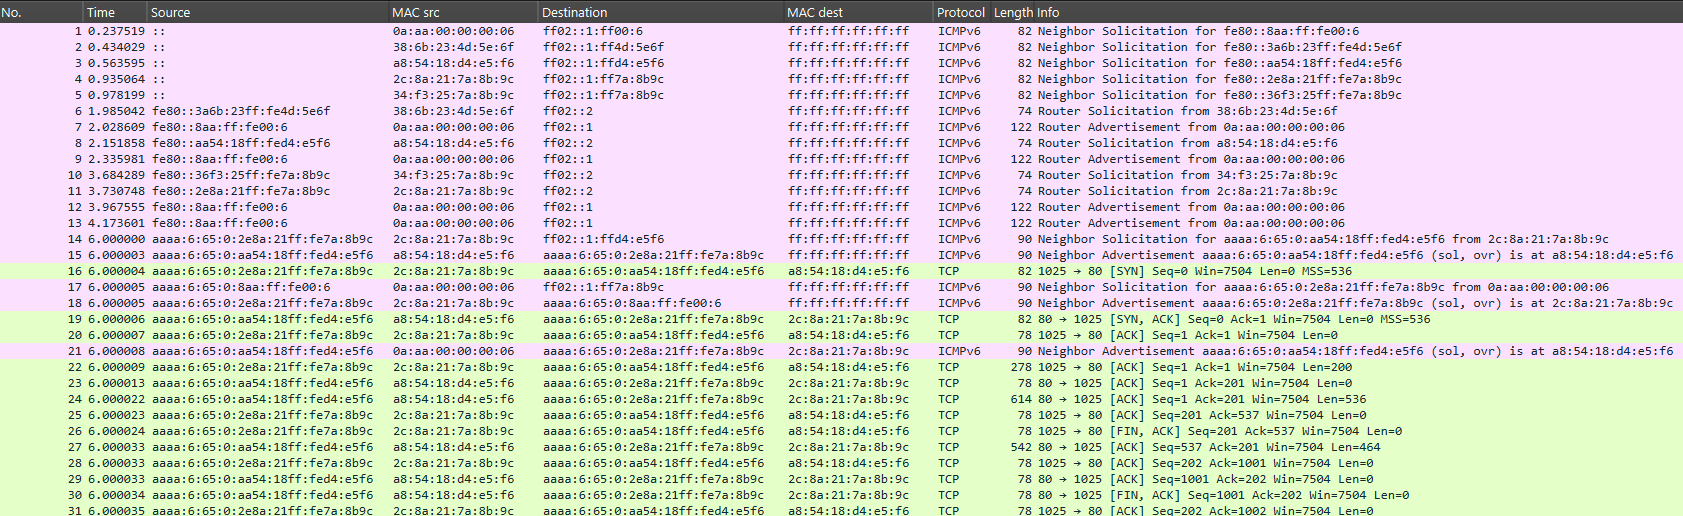
\includegraphics[width=135mm, scale=0.75]{imaxes/ejercicio2_4_1.png}
    \caption{Captura de paquetes entrantes y salientes de host[0]}
    \label{fig:paquetes_IPv6_host0}
\end{figure}

\begin{figure}[H]
    \centering
    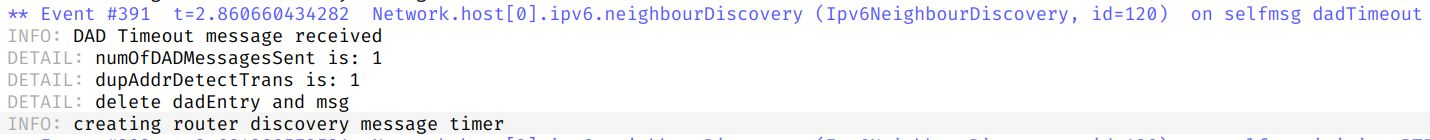
\includegraphics[width=135mm, scale=0.75]{imaxes/ejercicio2_4_2.png}
    \caption{Mensaje de fin de DAD para host[0]}
    \label{fig:DAD_host0}
\end{figure}

\begin{figure}[H]
    \centering
    \begin{lstlisting}
    lo0 ID:100 MTU:4470 UP LOOPBACK CARRIER macAddr:n/a Ipv6:{
        Addrs:::1(loopback)  expiryTime: inf prefExpiryTime: inf
        Node: dupAddrDetectTrans=1 reachableTime=36.455680949148
    }
    eth0 ID:101 MTU:1500 UP BROADCAST CARRIER MULTICAST macAddr:2C-8A-21-7A-8B-9C Ipv6:{
        Addrs:fe80::2e8a:21ff:fe7a:8b9c(link tent)  expiryTime: inf prefExpiryTime: inf
        mcastgrps:ff02::1 	Node: dupAddrDetectTrans=1 reachableTime=40.327972322702
    }
    \end{lstlisting}
    \caption{Tabla de interfaces de host[0] en t=0}
    \label{fig:InterfaceTableInicial}
\end{figure}

\begin{figure}[H]
    \centering
    \begin{lstlisting}
    lo0 ID:100 MTU:4470 UP LOOPBACK CARRIER macAddr:n/a Ipv6:{
	    Addrs:::1(loopback)  expiryTime: inf prefExpiryTime: inf
 	    Node: dupAddrDetectTrans=1 reachableTime=36.455680949148
   }

   eth0 ID:101 MTU:1500 UP BROADCAST CARRIER MULTICAST macAddr:2C-8A-21-7A-8B-9C Ipv6:{
	Addrs:fe80::2e8a:21ff:fe7a:8b9c(link)  expiryTime: inf prefExpiryTime: inf
	mcastgrps:ff02::1 	Node: dupAddrDetectTrans=1 reachableTime=40.327972322702
   }
    \end{lstlisting}
    \caption{Tabla de interfaces de host[0] en t=3}
    \label{fig:InterfaceTablePostDAD}
\end{figure}

\section{Ejercicio 2.5}
\subsection{¿En qué instante de la simulación obtienen los equipos sus direcciones IP globales? ¿Cómo obtienen esta
última? Muestra la tabla de interfaces de nodo host[0] en la que se vea su estado antes y después de obtener la
dirección global y explica qué cambia.}

Respecto a la captura de paquetes de la simulación realizada anteriormente ( Ver \ref{fig:paquetes_IPv6_host0} ), los equipos obtienen sus direcciones IP globales tras recibir un paquete de Router Advertisement. Como el primero en enviar un Router Solicitation es host[1] (Paquete número 6), es también el primero (Y único) que puede procesar el RA siguiente, obteniendo su dirección global en t=2.02. Después, ocurre lo mismo con server\_local, que obtiene su dirección en t=2.33, y con server\_remote, que la obtiene en t=2.72 (No se ve en \ref{fig:paquetes_IPv6_host0} porque server\_remote está en otra red). Finalmente, y como se observa parcialmente en \ref{fig:global_host0}, host[0] y host[2] obtienen la dirección global en t=2.72. Ambos la obtienen casi a la vez porque ambos emiten el paquete de Router Solicitation casi a la vez, de forma que, aunque el router devuelve dos paquetes RA, ambos obtienen la dirección global ya al recibir el primero. \\
Como se ha explicado en parte anteriormente, el proceso de obtener la dirección global comienza con un mensaje Router Solicitation del equipo al router correspondiente, enviado a la dirección multicast del grupo de los routers en el enlace local (FF02:02). En respuesta, el router responde un Router Advertisement en el que se anuncia junto con el prefijo global de la red correspondiente, que es con el que los nodos formarán su dirección global, a la dirección multicast de los nodos de la LAN (FF02::01). Los equipos que ya hayan enviado un paquete de RS pueden procesarlo, mientras que los que no lo hayan enviado o ya tengan una dirección global establecida, no. \\
Ahora, observando la tabla de interfaces de host[0] en \ref{fig:InterfaceTablePostGlobal}, observamos que una nueva dirección ha aparecido en la interfaz eth0, con la especificación \textit{global}, que se ha formado uniendo el prefijo global del red proporcionado por el router y la dirección MAC del dispositivo tras aplicar el proceso EUI-64, y a la que se le establece un tiempo de caducidad tras el que el equipo deberá volver a enviar un RS al router continuar teniendo una dirección global. Esta dirección es la que permite al dispositivo identificarse de forma única en Internet.

\begin{figure}[H]
    \centering
    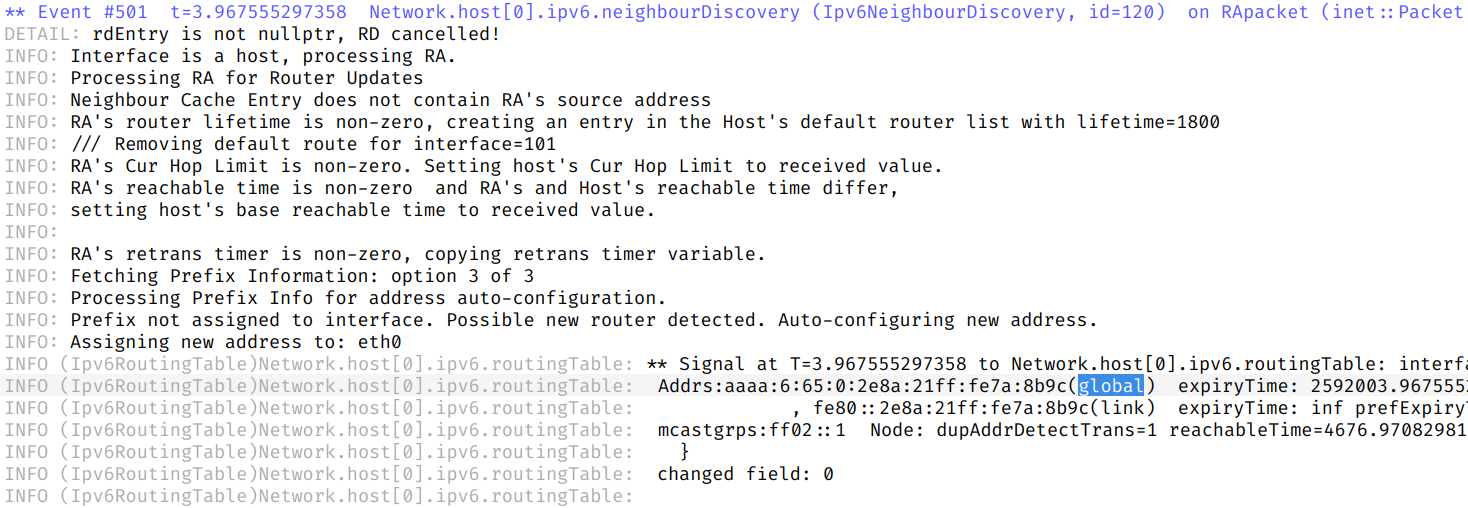
\includegraphics[width=135mm, scale=0.75]{imaxes/ejercicio2_5_1.png}
    \caption{Evento de obtención de dirección global para host[0]}
    \label{fig:global_host0}
\end{figure}

\begin{figure}[H]
    \centering
    \begin{lstlisting}
        lo0 ID:100 MTU:4470 UP LOOPBACK CARRIER macAddr:n/a Ipv6:{
            Addrs:::1(loopback)  expiryTime: inf prefExpiryTime: inf
            Node: dupAddrDetectTrans=1 reachableTime=36.455680949148
        }
        eth0 ID:101 MTU:1500 UP BROADCAST CARRIER MULTICAST macAddr:2C-8A-21-7A-8B-9C Ipv6:{
            Addrs:fe80::2e8a:21ff:fe7a:8b9c(link)  expiryTime: inf prefExpiryTime: inf
            mcastgrps:ff02::1 	Node: dupAddrDetectTrans=1 reachableTime=40.327972322702
        }
    \end{lstlisting}
    \caption{Tabla de interfaces de host[0] en t=3}
    \label{fig:InterfaceTablePostLocal}
\end{figure}

\begin{figure}[H]
    \centering
    \begin{lstlisting}
        lo0 ID:100 MTU:4470 UP LOOPBACK CARRIER macAddr:n/a Ipv6:{
            Addrs:::1(loopback)  expiryTime: inf prefExpiryTime: inf
                Node: dupAddrDetectTrans=1 reachableTime=36.455680949148
        }
        eth0 ID:101 MTU:1500 UP BROADCAST CARRIER MULTICAST macAddr:2C-8A-21-7A-8B-9C Ipv6:{
            Addrs:aaaa:6:65:0:2e8a:21ff:fe7a:8b9c(global)  expiryTime: 2592003.967555297358 prefExpiryTime: 604803.967555297358, 	
            fe80::2e8a:21ff:fe7a:8b9c(link)  expiryTime: inf prefExpiryTime: inf
            mcastgrps:ff02::1 	Node: dupAddrDetectTrans=1 reachableTime=4609.905032347888
        }
    \end{lstlisting}
    \caption{Tabla de interfaces de host[0] en t=4}
    \label{fig:InterfaceTablePostGlobal}
\end{figure}

\section{Ejercicio 2.6}
\subsection{Explica cómo se construye la IP global usando el nodo host[0] como ejemplo, de nuevo usando la notación
IPv6 no abreviada}

Una vez que el equipo manda un mensaje ICMPv6 con mensaje NS (Neighbor Solicitation) y no ocurre ningún fallo (No hay conflicto de IPs), procede a mandar un paquete ICMPv6 con mensaje RS (Router Solicitation), para que el router le asigne una IPv6 global (Este tipo de IPs ya son enrutables y únicas a nivel global). El router contesta con un paquete ICMPv6 con mensaje RA (Router Advertisement) indicando el prefijo global de red (Los primeros 64 bits de la dirección de la red al que está conectada host[0], en este caso AAAA:0006:0065:0000). Una vez que el host[0] obtiene el prefijo de la red, construye su IPv6 global substituyendo el prefijo de red del enlace local por la de la red, quedando su dirección como: AAAA:0006:0065:0000:2E8A:21FF:FE7A:8B9C. Esto se puede ver en la imagen \ref{fig:ip_global_host0}.

\begin{figure}[H]
    \centering
    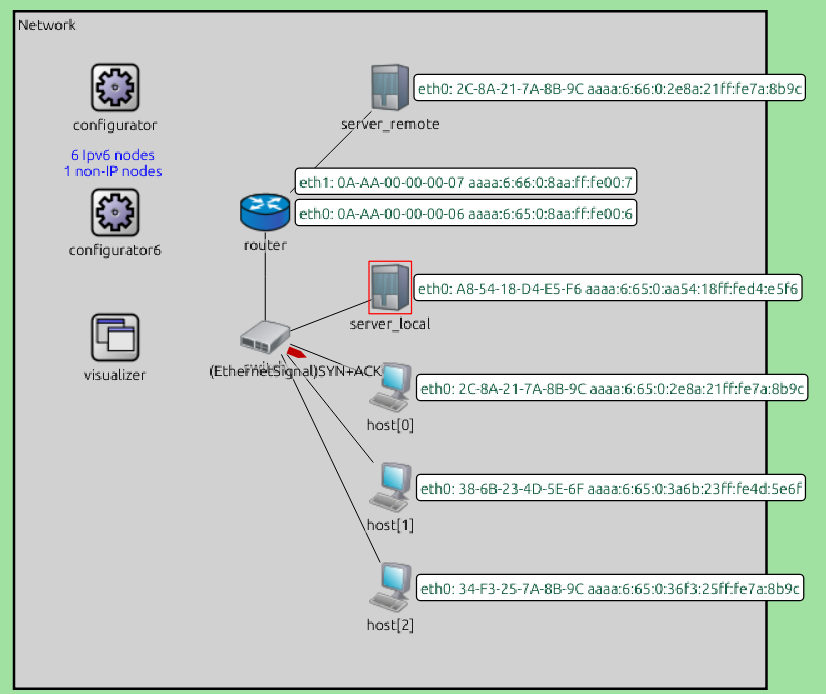
\includegraphics[width=135mm, scale=0.75]{imaxes/captura_ejer2_6.png}
    \caption{Foto red con direcciones IPv6 globales asignadas}
    \label{fig:ip_global_host0}
\end{figure}

\section{Ejercicio 2.7}
\subsection{Configura host[0] para que se conecte al servidor server remote usando su dirección fe80::x:x:x:x:
(asegúrate de que la dirección MAC de server remote es única). ¿Qué ocurre? Repite lo mismo para
server local. ¿Qué ocurre?}

Para realizar este ejercicio, se aplicaron los cambios descritos en la figura \ref{fig:conf_linklocalTCP} sobre la TcpBasicClientApplication de host[0], de forma que se conectara a los servidores directamente a tarvés de su dirección de enlace local.\\
En primer lugar, probamos la conexión a server\_remote. Como se observa en la figura \ref{fig:conexion_serverRemote}, host[0] no recibe el ACK correspondiente a ninguno de sus paquetes de intento de conexión. La primera vez que intenta la conexión, no recibe respuesta, por lo que lo intenta de nuevo una y otra vez enviando TCP Retransmisions. Esto es debido a que server\_remote se encuentra en una LAN distinta a host[0], que intenta alcanzar su dirección de enlace local. Los routers en IPv6 no enrutan paquetes como lo hacen en IPv4 entre redes, por lo que la única forma que tendría host[0] de completar la conexión sería usando la dirección unicast global del servidor.\\
Por otra parte, descubrimos que al realizar la conexión con server\_local, ocurre lo mismo ( \ref{fig:conexion_serverLocal} ). Esto es debido a un comportamiento propio de INET, que limpia de la tabla de enrutamiento la dirección local de enlace ( \ref{fig:fallo1} ) que permite conectarse a otros dispositivos en el mismo segmento de red después de recibir el prefijo de red del router ( \ref{fig:fallo2} ). En la realidad, la conexión al servidor local sí debería realizarse con éxito, ya que está en la misma LAN que host[0] y debería poder descubrirlo en el proceso de Neighbor Discovery.

\begin{figure}[H]
    \centering
    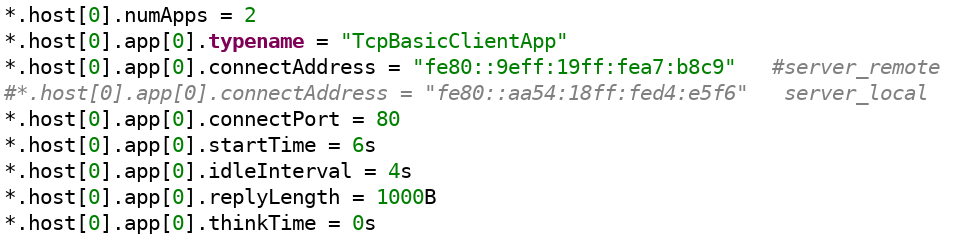
\includegraphics[width=135mm, scale=0.75]{imaxes/ejercicio2_7_1.png}
    \caption{Configuración establecida para este ejercicio}
    \label{fig:conf_linklocalTCP}
\end{figure}

\begin{figure}[H]
    \centering
    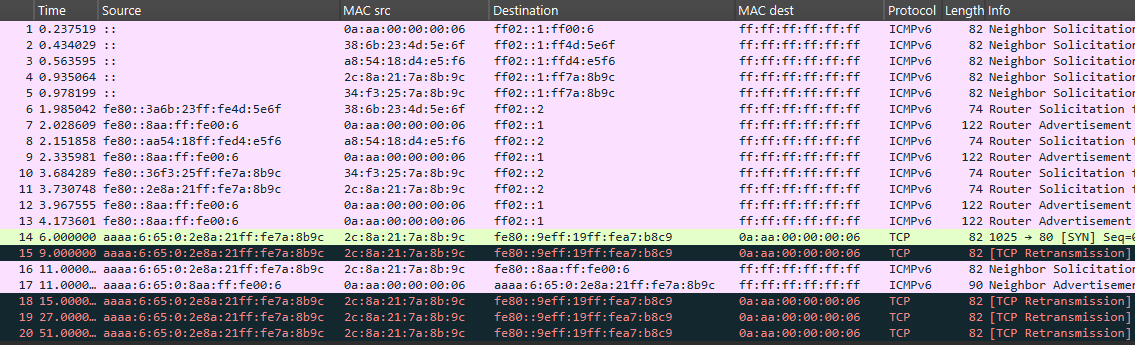
\includegraphics[width=135mm, scale=0.75]{imaxes/ejercicio2_7_3.png}
    \caption{Captura de paquetes en la conexión host[0] a server\_remote}
    \label{fig:conexion_serverRemote}
\end{figure}

\begin{figure}[H]
    \centering
    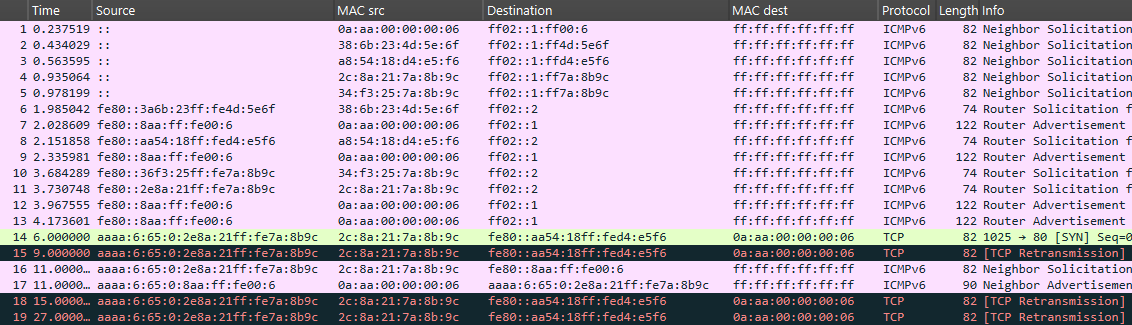
\includegraphics[width=135mm, scale=0.75]{imaxes/ejercicio2_7_2.png}
    \caption{Captura de paquetes en la conexión host[0] a server\_local}
    \label{fig:conexion_serverLocal}
\end{figure}

\begin{figure}[H]
    \centering
    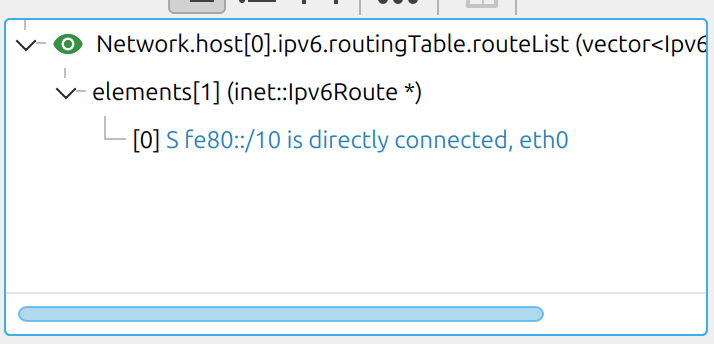
\includegraphics[width=65mm, scale=0.75]{imaxes/fallo1.png}
    \caption{Routing table de host[0] al inicio de la simulación}
    \label{fig:fallo1}
\end{figure}

\begin{figure}[H]
    \centering
    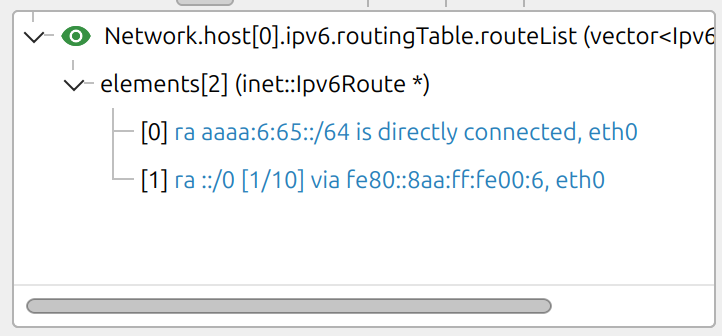
\includegraphics[width=65mm, scale=0.75]{imaxes/fallo2.png}
    \caption{Routing table de host[0] tras obtener la dirección unicast global}
    \label{fig:fallo2}
\end{figure}
